\documentclass{article}

\pdfpagewidth 8.5in
\pdfpageheight 11in

% \setlength\topmargin{0in}
% \setlength\headheight{0in}
% \setlength\headsep{0in}
% \setlength\textheight{7.7in}
\setlength\textwidth{6.5in}
\setlength\oddsidemargin{0in}
\setlength\evensidemargin{0in}
% \setlength\parindent{0.25in}
% \setlength\parskip{0.25in} 

\usepackage{makeidx}
\makeindex
\usepackage[dvips]{graphicx}

\usepackage{url}

\pagestyle{headings}

\author{Geoff Lawler \url{<geoff.lawler@cobham.com>} \and {Michael Elkins \url{<michael.elkins@cobham.com>}}}

\title{Watcher User's Guide}

\begin{document}
\maketitle
\newpage 

\tableofcontents
\newpage

\section{Introduction}

The {\it watcher}, or {\it watcher system} allows users to visualize emulated Mobile As-Hoc Networks. 

\section{General Watcher Information}
\subsection{Watcher Architecture and Communications}

Figure \ref{fig:watcherArch} shows the three main components in the watcher system: test node daemons (or ``feeders''), a watcher
daemon, and a number of graphical user interfaces (or ``GUIs''). The basic operation is this: the test nodes feed state 
information to a running instance of the watcher daemon, {\it watcherd}. The watcher daemon saves all the state information
locally to a database. A GUI connects to a running watcher daemon and requests a stream of state information, then displays it
using some (most likely) graphical mechanism. The daemon acts as a message cache and demulitplexer, streaming multiple
message streams from multiple test nodes into a single stream of messages. 

The interface between the watcher daemon and the test node is a simple message interface. The test node daemon connects
to a daemon, sends one or more messages, then disconnects. Some messages contain abstract state information about that test node
such as current set of neighbors, current location, etc. Other messages contain lower-level graphical display commands like ``change
color'' or ``draw an egde between these two nodes''.  For a list of all supported message, see the {\it watcher::event::Message} class 
documentation in the watcher developer documention. 

The interface between the GUI(s) and the watcher daemon is also message based, but also includes the concept of a message
stream. The stream is composed of messages and has an interface that manipulates the stream content, time, direction, and rate. A message
stream can start at any time {\it t} for which there is data. The stream rate can be set as a multipler of real time. For instance
a GUI can request that the stream go 10x the speed at which the messages were received. (This only will work od course if there is 
a cache of messages that can be sent at 10x - once the message cache is exhausted, the stream is sent at the rate the messages
are recieved, 1x real time.) 

There are three modes the system can be run in, ``record mode,'' ``live mode,'' and ``playback mode''. In ``record'' mode, These modes
can be moved into and out of in real time depending on the needs of the user. In record mode, the test nodes and a watcher daemon are
run. The test nodes send state data to the daemon, the the daemon writes those messages to a local database. In live mode, the test 
nodes are feeding data to the daemon (which writes the information to a database) and some number of GUIs connect to the 
daemon and request a message stream. Note that the GUIs can request messages from the start of the test run - thay are not
contrained to ``live'' messages; live mode simply means that there are, at that moment, new messages arriving at the daemon
and being recorded. The last mode os playback mode and does not involve test node daemons. In this mode, the watcher daemon
is started with an existing database full of messages and it just waits for connections from a GUI. When a GUI connects, the 
watcher daemon streams it the requested messages, this ``playing back'' a ``recorded'' test run. 

\begin{figure}[here]
\label{fig:watcherArch}
\centering
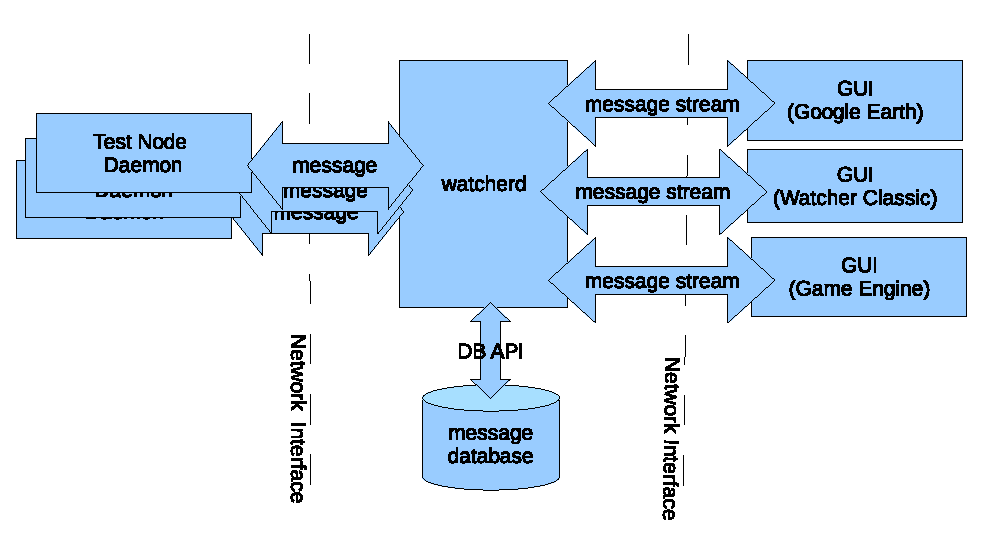
\includegraphics[width=0.8\textwidth]{watcherArch.eps}
\caption{The basic architecture of the watcher system.}
\end{figure}

\subsection{Obtaining and Building Watcher}
Mention GPL'd-ness of the watcher. Give reference to repo location. 

Give list of dependencies.

Give simple build instructions: ./autogen.sh, ./configure, make, sudo make install, cd clients/legacyWatcher, make, make install \ldots.

\subsection{Log Property Files}
Give general intro with examples of the standard format and workings of the log.properties file. (Just like Java if peeps know that.)

\subsection{Configuration (cfg) Files} 
explain layout of standard config files and arguments that most (all?) watcher modules understand (-f cfg). 

\subsection{Command Line Arguments}
Most binaries take a {\tt -c} (or {\tt -f}) arugment which gives the location of the {\tt cfg} file. Mention this. Also note that most binaries 
just take that option and nothing else. 

\section{Test Node Components}
\subsection{Watcher API}
Mention watcher messages and give types. Mention something else that's interesting and useful. 

\subsection{Scripting Interface}
For each watcher message there is a command line binary to send that message. These binaries can be used directly in shell scripts or invoked via a system call from most scripting languages to send 
an instance of that message to a running watcher daemon instance. Each binary allows the user to specify the content of the message and the daemon instance to send the message to. 

In many cases, the node that the message ``comes from'' can be set as well. This allows a user on any machine that can connect to a watcher daemon, the ability to modify nodes, edges, lables, etc of any 
test node. This is useful for debugging or real time modification of an aspect of the test bed. For instance a single machine could monitor traffic rates between nodes and update 
the edges between those nodes with the current traffic rate. 
\\\\
The available commands are:
\begin{itemize}
\item sendColorMessage (page \pageref{sendColorMessage})
\item sendEdgeMessage (page \pageref{sendEdgeMessage})
\item sendGPSMessage (page \pageref{sendGPSMessage})
\item sendConnectivityMessage (page \pageref{sendConnectivityMessage})
\item sendDataPointMessage (page \pageref{sendDataPointMessage})
\item sendLabelMessage (page \pageref{sendLabelMessage})
\item showClock (page \pageref{showClock})
\end{itemize}
The following pages give details for each command.
\newpage
\label{sendColorMessage}
\subsubsection{sendColorMessage}
{\bf sendColorMessage} is a test node command line program that sends a ColorMessage message to the watcher daemon, specifing that a node should change it's color. 
\\\\
Usage: 
{\tt sendColorMessage -s server -c color [optional args]}
\\\\
Required Arguments:
\begin{itemize}
\item {\tt -c, --color=color}, The color of the node. Can be ROYGBIV or RGBA format, string or hex value. Supports transparency. 
\item {\tt -s, --server=address}, The addres of the node running watcherd
\end{itemize}
Optional Arguments:
\begin{itemize}
\item {\tt -n, --node=address}, The node to change color, if empty the local node's address is used
\item {\tt -f, --flash=milliseconds}, Flash between the new color and the orginal color every milliseconds seconds, 0 for no flash.
\item {\tt -x, --expiration=seconds}, How long in seconds to change the color. 0==forever
\item {\tt -p, --logProps}, log.properties file, which controls logging for this program
\item {\tt -h, --help}, Show help message
\end{itemize}
Examples:
\begin{itemize}
\item This tells the GUI(s) that are listening to the daemon running node {\em glory} the node at 192.168.1.101 should be drawn in blue:

{\tt sendColorMessage -s glory -c blue -n 192.168.1.101}

\item This tells the GUI(s) that are listening to the daemon running node {\em glory} the node at 192.168.1.101 should be drawn in a transparent blue. 
Transparent format is R.G.B.A, where {\em A} is alpha transparency:

{\tt sendColorMessage -s glory -c 0.0.255.64 -n 192.168.1.101}
  
\item This tells the GUI(s) that are listening to the daemon running node {\em glory} the node at 192.168.1.107 should be drawn in green for 5 seconds:
 
{\tt sendColorMessage -s glory -c green -n 192.168.1.107 --expiration 5000}
 
\item This tells the GUI(s) that are listening to the daemon running node {\em glory} the node at 192.168.1.104 should flash for 10 seconds:
 
{\tt sendColorMessage --server glory --color green --node 192.168.1.104 --flash --expiration 10000}

\end{itemize}

\newpage
\label{sendEdgeMessage}
\subsubsection{sendEdgeMessage}

{\bf sendEdgeMessage} is a test node command line program that sends a GPSMessage message to a watcher daemon, specifing a node's current GPS coordinates.
\\\\
Usage: 
{\tt sendEdgeMessage -s server -t tail [optional args]}
\\\\
Required Arguments:
\begin{itemize}
\item {\tt -s, --server=address}, The address or name of the node running watcherd to which the message is sent.
\item {\tt -t, --tail=address}       The node to attach the tail of the edge to. If no head is given, the local node is used.
\end{itemize}
Optional Arguments:
\begin{itemize}
\item {\tt -h, --head=address}       The node to attach the head of the edge to.
\item {\tt -c, --color=color}        The color of the edge. Can be ROYGBIV or RGBA format, string or hex value. Supports transparent colors.
\item {\tt -w, --width=width}        The width of the edge in some arbitrary, unknown unit.
\item {\tt -y, --layer=layer}        Which layer the edge is on in the GUI.
\item {\tt -d, --bidirectional=bool} Is this edge bidirectional or unidirectional. Use 'true' for true, anything else for false.
\item {\tt -l, --label=label}        The text to put in the middle label (This program only supports creating a middle label, although the message supports labels on node1 and node2 as well. May add that later)
\item {\tt -f, --labelfg=color}      The foreground color of the middle label. Can be ROYGBIV or RGBA format, string or hex value. Supports transparent colors.
\item {\tt -b, --labelbg=color}      The background color of the middle label. Can be ROYGBIV or RGBA format, string or hex value. Supports transparent colors.
\item {\tt -z, --fontSize=size}      The font size of the middle label
\item {\tt -x, --expiration=seconds} How long in milliseconds to diplay the edge
\item {\tt -p, --logProps}           log.properties file, which controls logging for this program
\end{itemize}
Examples:
\begin{itemize}
\item Draw an edge between node 101 and node 102 on the "QoS" layer and make the color a translucent red.

{\tt sendEdgeMessage -s glory -h 192.168.1.101 -t 192.168.1.102 -l QoS -c 255.0.0.64}
\end{itemize}


\newpage
\label{sendGPSMessage}
\subsubsection{sendGPSMessage}
{\bf sendGPSMessage} is a test node command line program that sends a GPSMessage message to a watcher daemon, specifing a node's current GPS coordinates.
\\\\
Usage: 
{\tt sendGPSMessage -s server -x value -y value -z value [optional args]}
\\\\
Required Arguments:
\begin{itemize}
\item {\tt -s, --server=address}, The address or name of the node running watcherd to which the message is sent.
\item {\tt -x, --latitude=value}, The latitude of the node.
\item {\tt -y, --longitude=value}, The longitude of the node.
\item {\tt -z, --altitude=value}, The altitude of the node.
\end{itemize}
Optional Arguments:
\begin{itemize}
\item {\tt -n, --fromNode=address|name}, The node that the coordinates refer to. If not given, assume the local node. 
\item {\tt -l, --logProps}, log.properties file, which controls logging for this program
\item {\tt -h, --help}, Show help message
\end{itemize}
Examples:
\begin{itemize}
\item This tells the GUI(s) attached to the watcherd on glory that node 192.168.1.101 is now at 79.23123123, 43.123123123, 20

{\tt sendGPSMessage -s glory -n 192.168.1.101 -x 79.23123123 -y 43.123123123 -z 20}

\item This tells the GUI(s) attached to the watcherd on glory that the local node is at 0.0123123 0.123123123 123

{\tt sendGPSMessage --server glory -n 192.168.1.101 -x 0.0123123 -y 0.123123123 -z 123}

\end{itemize}

\newpage
\label{sendConnectivityMessage}
\subsubsection{sendConnectivityMessage}
{\bf sendConnectivityMessage} is a test node command line program that sends a watcher::event::ConnectivityMessage message to the watcher daemon, specifying the current list of neighbors that the node has. 
The GUI(s) that are listening to that daemon, then draw the neighbors in a way that is relevent for that particular GUI.
\\\\
Usage: 
{\tt showColor -s server [optional args] nbr1 nbr2 nbr3 ... nbrN}
\\\\
Required Arguments: 
\begin{itemize}
\item {\tt -s, --server=address}, The addres of the node running watcherd.
\item {\tt nbr1 nbr2 nbr3 ... nbrN} - the list if neighbors by ipaddress.
\end{itemize}
Optional args:
\begin{itemize}
\item {\tt -l, --layer=layer}, the layer that these neighbors should show up on when displayed in the GUI(s).
\item {\tt -p, --logProps=log.propertiesFile}, the log properties file to use.
\item {\tt -f, --fromNode=fromNodeAddr}, the node that has these neighbors, if not given the local node is assumed.
\end{itemize}
Examples:
\begin{itemize}

\item This tells the GUI(s) that are listening to the daemon running on 'glory' the local test node has neighbors 192.168.1.101 and 192.168.1.102

{\tt sendConnectivityMessage -s glory 192.168.1.101 192.168.1.102}

\item This tells the GUI(s) that are listening to the daemon running on 'glory' the local test node 192.168.1.101 has neighbor nodes 192.168.1.110-192.168.1.115 and they should be displayed on the "children" layer. (Note that 192.168.1.11\{0..5\} is a bashism which expands to the sequenctial list of nodes 192.168.1.110-192.168.1.115.) 

{\tt sendConnectivityMessage -s glory -l children -f 192.168.1.101 192.168.1.11\{0..5\}i}

\end{itemize}

\newpage
\label{sendDataPointMessage}
\subsubsection{sendDataPointMessage}
{\bf sendDataPointMessage} is a test node command line program that sends a DataPointMessage message to the watcher daemon, specifing a set of timestamped data point(s) for the node. The data point is labeled with a string saying what the data points represent.  The GUI(s) then display this information is some way. In the case of the legacy watcher [\ref{LegacyWatcher}], 2D scrolling graphs are displayed showing past data points. The legacy watcher assumes that data points are given once a second.
\\\\
Usage: 
{\tt sendDataPointMessage -s server -g name [optional args] -d dp1 -d dp2 ... -d dpN}
\\\\
Required Arguments:
\begin{itemize}
\item {\tt -s address|name}, The address or name of the node running watcherd.
\item {\tt -g name}, the "graphname" of the data - what the data is measuring.
\item {\tt -d datapoint}, a single data point measuring something.
\end{itemize}
Optional args:
\begin{itemize}
\item {\tt -n, --node=address}, the node the data is from 
\item {\tt -h, --help}, Show help message
\end{itemize}
Examples:
\begin{itemize}
\item Update the watcher about the current CPU usage on the machine 192.168.1.105.  
    
{\tt sendDataPointMessage -s glory -g "CPUUsage" -n 192.168.1.105 -d .45432}

\item Update the watcher about the current number of user's logged in to the local machine.   

{\tt sendDataPointMessage -s glory -g "LoggedInUsers" -d 23}

\item Update the watcher about the local node's current level of self satisifation.

{\tt sendDataPointMessage -s glory -g "BoyAmIGreatLevel" -d 23}

\end{itemize}

\newpage
\label{sendLabelMessage}
\subsubsection{sendLabelMessage}
{\bf sendLabelMessage} is a test node command line program that sends a watcher::event::LabelMessage message to the watcher daemon, specifing that a label should be attached to the specified node (or float if given coords).

If address is specified, the label will attach to the node with that address. If cooridinates are
specified, the label will float at those coordinates. The node address takes precedence. If neither
option is specified, the label will attach to the node from which the message saw sent.
\\\\
Usage: 
{\tt sendLabelMessage -s server -l label [optional args]}
\\\\
Required Arguments:
\begin{itemize}
\item {\tt -l, --label=text}, The text of the label
\item {\tt -s, --server=address}, The address|name of the node running watcherd, the server.
\end{itemize}
Optional args:
\begin{itemize}
\item {\tt -n, --node=address}, The node to change color, if empty the local node's address is used
\item {\tt -x, --latitude=coord}        The latitude to float the node at.
\item {\tt -y, --longitude=coord}       The longitude to float the node at.
\item {\tt -z, --altitiude=coord}       The altitude to float the node at.
\item {\tt -t, --fontSize=size}         The font size of the label
\item {\tt -f, --foreground=color}      The foreground color of the label. Can be ROYGBIV or RGBA format, string or hex value.
\item {\tt -b, --background=color}      The background color of the label. Can be ROYGBIV or RGBA format, string or hex value.
\item {\tt -e, --expiration=seconds}    How long in millisecond to diplay the label
\item {\tt -r, --remove}                Remove the label if it is attached
\item {\tt -L, --layer=layer}           Which layer the label is part of. Default is "Physcial".
\item {\tt -x, --expiration=seconds}, How long in seconds to change the color. 0==forever
\item {\tt -p, --logProps}, log.properties file, which controls logging for this program
\item {\tt -h, --help}, Show help message
\end{itemize}

Examples:
\begin{itemize}

\item sendLabelMessage -s glory -n 192.168.1.102 -l "Correlation Layer" -e 1500 -f red -b green -L Correlation
\item sendLabelMessage -s glory -n 192.168.1.102 -l "Physical Layer" -e 1500 -L Physical
\item sendLabelMessage -s glory -n 192.168.1.104 -l "Attack Detected" -f yellow -b blue -L Physical 

\end{itemize}


\newpage
\label{showClock}
\subsubsection{showClock}

{\bf showClock} is a command line program that ``draws'' a clock by arranging a set of nodes and edges into the shape of an 
analog clock.  The ``clock'' is updated once a second to move ``the hands'' of the clock around. This program is mostly
used to test the TiVO-like functionality built into the watcher system. But it can also be used to simply test if the watcher system is working properly. It does not need to be run on a test node - it is generally run on the same machine as the watcher daemon is running, but of course does not have to be. An example can be seen in Figure ~\ref{fig:LegacyWatcherClock} on page \pageref{LegacyWatcher}.
\\\\
Usage: 
{\tt showClock -s server [optional args]}
\\\\
Required Arguments:
\begin{itemize}
\item {\tt -s, --server=address|name}, The address or name of the node running watcherd
\end{itemize}
Optional Arguments:
\begin{itemize}
\item {\tt -r, --radius}, The radius of the clock face in some unknown unit
\item {\tt -S, --hideSecondRing}        Don't send message to draw the outer, second hand ring.
\item {\tt -H, --hideHourRing}          Don't send message to draw the inner, hour hand ring.
\item {\tt -p, --logProps=file}, log.properties file, which controls logging for this program
\item {\tt -e, --expireHands}           When drawing the hands, set them to expire after a short time.
\item {\tt -h, --help}, Show help message
\end{itemize}
Examples:
\begin{itemize}
\item This shows a clock with a radius or 10 units.

{\tt showClock -s glory -r 10}

\item This shows a clock with a radius or 10 units, but no outside minute ring and the edges which make up the hands are refreshed every second.

{\tt showClock --server glory --radius 10 --hideHourRing --expireHands}

\end{itemize}


\subsection{Test Node Daemons}
These daemons are run on the test nodes and feed information about the test nodes to the watcher daemon. This information is then streamed to GUI(s) attached to the daemon, which display it.
\subsubsection{GPS Feeder}
\label{GPSFeeder}
The GPS Feeder, {\it gpsFeeder.py}, updates the watcher daemon on the current location of a single node on the test bed. It is usually run on the test node itself, thus 
every test node updates its own location. The GPS is read from a locally running {\it gpsd} process. (See http://gpsd.berlios.de for 
details of {\it gpsd}.) The watcher GPS Feeder can be found at ./src/clients/gpsFeeder. It consists of a python script that uses the 
python interface exported by {\it gpsd}. Once a second, it retrieves the curent GPS location of the local node and makes a system call via the shell to sendGPSMessage ~\ref{sendGPSMessage}. (Since it
calls {\it sendGPSMessage}, {\it sendGPSMessage} must be in the PATH of the shell in which gpsFeeder is launched. 
\\\\
Usage: 
{\tt gpsFeeder -s server}
\\\\
Required Arguments:
\begin{itemize}
\item {\tt -s,--server=address|name}, The address or name of the node running watcherd.
\end{itemize}
Example:
\begin{itemize}
\item Run the gpsFeeder to give current location information to the watcher daemon once a second and save the output as a log to {\tt /var/log/gpsFeeder.log}.
    
{\tt gpsFeeder.py -s glory 2>\&1 /var/log/gpsFeeder.log}
\end{itemize}

Note: the {\it emane} system uses the gpsd from gpsd.berlios.de and this is the daemon that the gps feeder supports. There is an older {\it gpsDaemon} that supports a {\it MANE} environment, but that 
is not supported directly by this watcher system release. Use the unsupported {\it gpsDaemon} and the auxillary program {\it watcherHierarchyClient} (see page \pageref{watcherHierarchyClient}) for {\it MANE} support in this release 
of the watcher system.

There are plans to create a global GPS Feeder that would feed all location information to the watcher daemon directly in order to cut down on network traffic, which 
would be very useful once the watcher is run on a system with hundreds or thousands of nodes. But these are still just plans. 


\subsubsection{watcherHierarchyClient}

The {\it watcherHierarchyClient} daemon is used to support a test bed running the the dynamic hierarchy software. 
The watcher was orgininally written with the hieracht daemons as a transport layer and as part of a 
dynamic hierarchy MANET platform. Thus the {\it watcherHierarchyClient} daemon is used for backwards compatibility. 
The basic idea of the {\tt watcherHierarchyClient} is that it connects to a hierarchy instance, subscribes
to all the messages that a watcher GUI may care about and when it receives such a message it translates it 
into something that the (new) watcher system can understand. 

{\it watcherHierarchyClient} is the glue between hierachy land and watcher land. {\it watcherHierarchyClient}, when started, connects
to a running hierarchy daemon and subscribes to all watcher related messages. When it receives a watcher related
messages, it converts the message into something the watcher system can understand and sends it to the watcher daemon
that it is connected to. {\it watcherHierarchyClient} is meant to offer backward compatibility to all "old style" watcher 
clients. It acts as a go-between between old hierarchy messages and the new watcher messages.
\\\\
Usage:
{\tt watcherHierarchyClient -s watcher\_daemon\_name\_or\_address -u hierachy\_daemon\_node\_address}
\\\\
Arguments:
\begin{itemize}
\item {\tt -s}, The address or name of the node running the watcher daemon, watcherd.
\item {\tt -u}, The address of the node running the hierachy daemon.
\end{itemize}



\newpage
\label{watcherd}
\section{The Watcher Daemon}

The watcher daemon is responsible for collecting events from the test nodes and
sending event streams to the Watcher GUIs.  Events from the test nodes are
stored in an SQLite databased (named "event.db" by default).  The Watcher Daemon
determines whether a connection is a test node or GUI by the type of the first
event received.

When recording events from the test nodes into the database, events are
appended to the existing database, or a new database is created if it does not
exist.  The Watcher Daemon may also be invoked in read-only database mode using
the command line option {\tt -r} or {\tt --read-only}, in which case events are not stored
in the database.  Read-only mode is useful particularly when replaying events
from a database from some time in the past.  In this case, it may not make
sense to append any current event stream from the test nodes when a large time
gap exists between past and present runs.

The watcher daemon source code can be found in {\tt .\slash src\slash watcherd}. The binary produced after building is 
named {\tt watcherd}. 

\subsection{Live Mode}

When a GUI connects to the Watcher Daemon, it will by default subscribe to the
live event stream coming from the test nodes.  In this case, the Watcher Daemon
is simply retransmitting received events to all listening GUIs rather than
fetching events from the database.  The events are also stored in the database
for later replay.

If a GUI pauses, rewinds, or slows playback, it will switch to Playback mode.

\subsection{Playback Mode}

In Playback Mode, the Watcher Daemon fetches events from the database and sends
them to the GUI.  Each GUI connection has an independent notion of the current
playback time offset, direction and speed.  Stopping playback in one GUI will
not cause playback to stop in another GUI.

The Watcher Daemon will automatically pause Playback when the last event from
the database has been sent to the GUI.  Thus, if a GUI were playing at a time
offset near the end of the database, and faster than real time, the GUI will be
paused when the last event is sent, even if additional events arrive from test
nodes.

\subsection{Configuration}

The Watcher Daemon has several optional configuration options.  By default,
watcherd will read its configuration from a file named {\tt watcherd.cfg}.  An
alternate configuration file can be specified using the {\tt -c} command line
option.

\begin{itemize}
\item {\tt server}, the DNS name or IP address of the network interface to listen for
connections
\item {\tt port}, the TCP port number to listen on for connections (default: 8095)
\item {\tt serverThreadNum}, the number of threads to spawn for handling connections
\item {\tt databasePath}, the full pathname to the test node event database (default:
{\tt event.db})
\item {\tt dataNetwork}, if it exists, this network address will be mapped onto any
incoming feeder messages that do not specify a source address. For example, if the 
{\tt dataNetwork} is set to 192.168.10.0 and the incoming feeder message is from ip address
192.168.1.121, the incoming feeder message is set to 192.168.10.121. This is needed as the watcher
daemon will use the ip address of incoming feeder messages to set the {\tt from address} on the messages.
If the watcherd is running on a network that is different than the test nodes (which is 
frequently the case when using a control network), this will map the control network addresses
to the data network address space, so all feeder messages appear to come from the same
network. If the dataNetwork was not specified, then this would generate 2 different
addresses for a single node, confusing any attached GUI.
\end{itemize}

\subsection{Command Line Options}

\begin{itemize}
\item {\tt -c} or {\tt --config}, specify an alternate configuration file (default: {\tt
watcherd.cfg})
\item {\tt -r} or {\tt --read-only}, mark the event database Read Only so that no
new events from test nodes will be written
\item {\tt -h} or {\tt --help}, display a list of all supported command line
options
\end{itemize}



\section{Watcher GUIs}

Talk about GUIs here. Legacy watcher is OpenGL, others are engine based and just barely started proof of concept.

\subsection{Legacy Watcher}
\label{LegacyWatcher}
\begin{figure}[here]
\label{fig:LegacyWatcherClock}
\centering
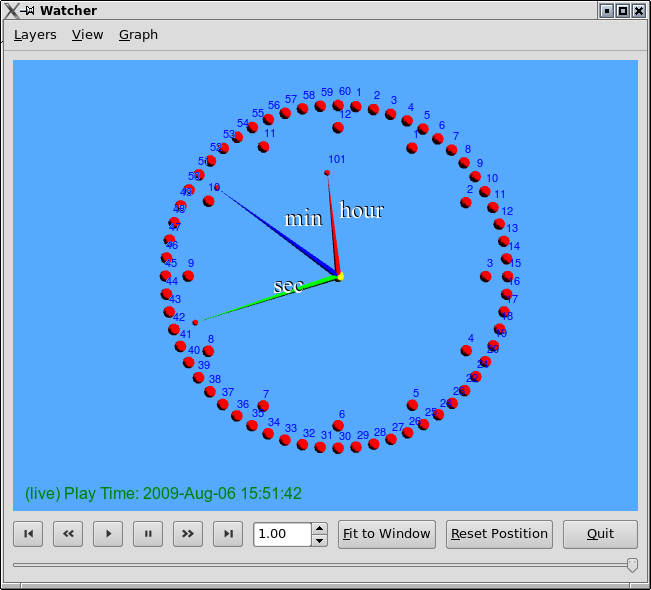
\includegraphics[width=0.8\textwidth]{legWatcherGUI.eps}
\caption{The legacy watcher showing a running instance of showClock.}
\end{figure}

\subsection{ogreWatcher}
\begin{figure}
\centering
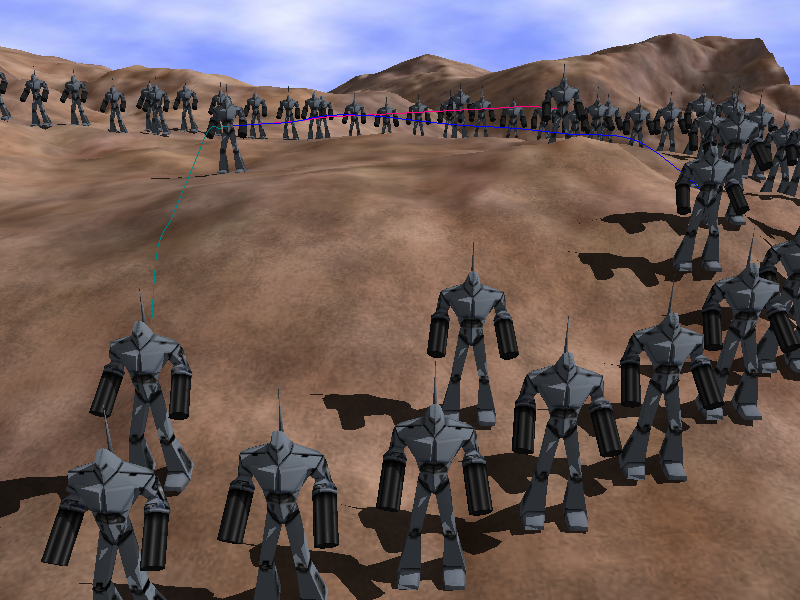
\includegraphics[width=0.8\textwidth]{ogreWatcherGUI.eps}
\caption{The ogreWatcher showing a running instance of showClock.}
\end{figure}

Built with OGRE.
\subsection{Watcher3d}
Built with Delta-3d.

\printindex

\end{document}
